\documentclass[12pt]{article}

\usepackage{xcolor}
\usepackage{graphicx}
\usepackage[left=1.5cm,top=2.5cm,right=1.5cm,bottom=2.5cm,bindingoffset=0.5cm]{geometry}

\usepackage{dsfont}
\usepackage{algorithm2e}
\usepackage{stmaryrd}
\usepackage{amsmath}
\usepackage[mathlines]{lineno}% Enable numbering of text and display math
\DeclareMathOperator{\Tr}{Tr}
\usepackage{url}
\usepackage[normalem]{ulem}
\usepackage{multicol, caption}
\usepackage{braket}
\bibliographystyle{elsarticle-num}

\makeatletter
\def\ps@pprintTitle{%
	\let\@oddhead\@empty
	\let\@evenhead\@empty
	\let\@oddfoot\@empty
	\let\@evenfoot\@oddfoot
}
\makeatother
\makeatletter
\makeatother

\newenvironment{Figure}
  {\par\medskip\noindent\minipage{\linewidth}}
  {\endminipage\par\medskip}

\begin{document}


\title{Matrix Product States}
%
%
% author names and IEEE memberships
% note positions of commas and nonbreaking spaces ( ~ ) LaTeX will not break
% a structure at a ~ so this keeps an author's name from being broken across
% two lines.
% use \thanks{} to gain access to the first footnote area
% a separate \thanks must be used for each paragraph as LaTeX2e's \thanks
% was not built to handle multiple paragraphs
%
\author{Glenn~LeBlanc,
Karthik~Siva
\thanks{This project was part of the Berkeley Physics Directed
Reading Program, which allows undergraduates to explore novel
material under the auspices of a graduate student mentor. K. Siva
very graciously directed this project.}}

\maketitle
\begin{multicols}{2}

\section*{Introduction}
	\subsection*{Many-Body Wavefunctions as Tensors}
		Consider a spin-$\frac{1}{2}$ particle. The particle's state is given by
		$\ket{\psi}\in\mathds{C}^2$, and for some computational basis
		$\{\ket{0}, \ket{1}\}$ we can write
		$$\ket{\psi}=\alpha\ket{0}+\beta\ket{1}$$
		with
		$$|\alpha|^2+|\beta|^2=1.$$
		This is the principle of superpostion-- the particle is superposed
		between the two basis states $\ket{0}$ and $\ket{1}$. Now if we add
		a second spin-$\frac{1}{2}$ particle, the many-body system
		$\ket{\Psi}$ is in some superposition of the four states
		$$\ket{\Psi}=\alpha\ket{00}+\beta\ket{01}+\gamma\ket{10}+\delta\ket{11}.$$
		Generally, for $N$ qubits (qudits) the system is fully
		parameterized by $2^N$ ($d^N$) complex numbers:
		$\ket{\Psi}\in\mathds{C}^{2^N}$. Notice the exponential scaling
		here. It is useful also to notice the natural bijection between
		the two spaces
		$$\mathds{C}^{2^N}\longleftrightarrow \mathds{C}^{2\times\cdots\times 2}$$
		meaning we can instead conceptualize $\ket{\Psi}$ as a
		\textit{tensor}:
		$$\ket{\Psi}\in\mathds{C}^{2\times\cdots\times2}$$
		where in this paper a tensor $\Psi$ is just a multidimensional
		array with some number of indices such that plugging in an
		assignment for each index spits out a complex number. More
		succinctly,
		$$\Psi_{i_1,i_2,\cdots,i_N}\in\mathds{C}$$
		A \textit{contraction} between two tensors $\Psi$ and $\Phi$ is
		a summation over a shared index:
		$$T_{i,j,l,m}=\sum_k\Psi_{i,j,k}\Phi_{l,k,m}$$
		is an example of a contraction. Note that dot products, matrix
		multiplication, and trace are all different vestiges of tensor
		contraction:
				\begin{align*}
				a\cdot b &=\sum_ka_kb_k\\
				(Ax)_{i} &=\sum_kA_{ik}x_k\\
				\Tr(A)&=\sum_kA_{kk}
			\end{align*}


	\subsection*{Tensor Networks}
	A \textit{tensor network} is an undirected graph whose nodes
	represent tensors and whose edges correspond to tensor indices. An
	edge between two tensors corresponds to a contraction along the
	depicted axis of each tensor. Use of this graphical language for
	representing quantum systems is attractive since it unveils relevant
	entanglement properties~\cite{TnIntro}.
	\begin{Figure}
		\center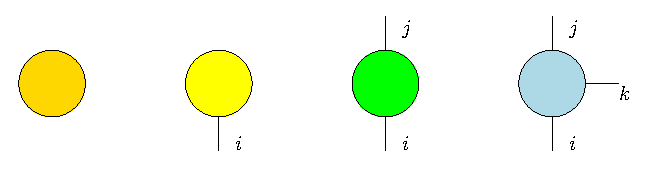
\includegraphics[width=.9\textwidth]{./Figures/tensors.eps}
		\captionof{figure}{\textit{A graphical depiction of a scalar $c$, vector
		    $v_i$, matrix $M_{ij}$, and a tensor $T_{ijk}$ of rank three.}}
		\label{tensor-graphics}
	\end{Figure}
	See figure~\ref{tensor-graphics} for a graphical depiction of
	tensors of rank zero to three. Each tensor is denoted as a node with
	free edges representing each index.

	Figure~\ref{tensor-contractions} depicts the previous examples (dot
	product, matrix multiplication, trace) of tensor contraction using
	this graphical language.
	\begin{Figure}
		\center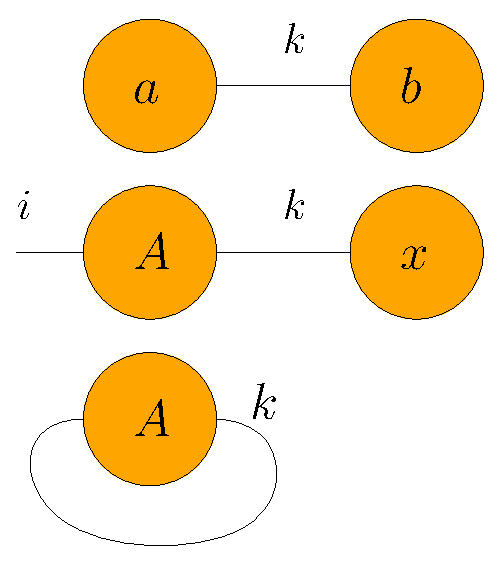
\includegraphics[width=.35\textwidth]{./Figures/contractions.eps}
		\captionof{figure}{\textit{A graphical depiction of three examples of
		    tensor contraction.}}
		\label{tensor-contractions}
	\end{Figure}
	An example of an insight this graphical language provides is in
	proving trace cyclicality. The standard proof is as follows:
	\begin{align*}
		\Tr(ABC)&=\sum_{ijk}A_{ij}B_{jk}C_{ki}\\
						&=\sum_{ijk}C_{ki}A_{ij}B_{jk}\\
						&=\Tr(CAB)
	\end{align*}
	The tensor network proof is depicted in figure~\ref{trace}:
	\begin{Figure}
		\center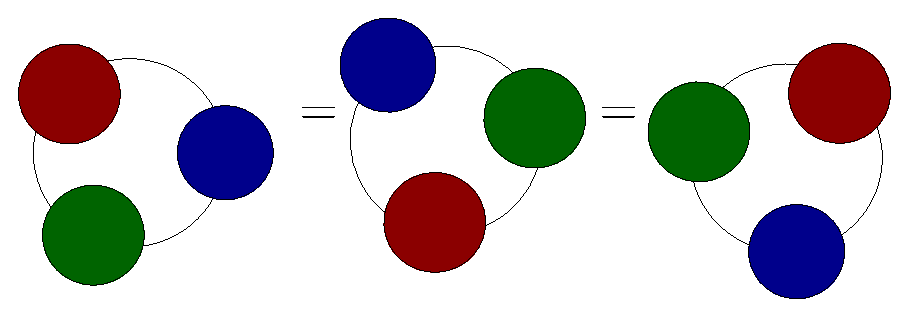
\includegraphics[width=.7\textwidth]{./Figures/trace.eps}
		\captionof{figure}{\textit{Proof of trace cyclicality.}}
		\label{trace}
	\end{Figure}
	The graphical depiction of trace provides simpler insight into the
	cyclic structure of the underlying tensor contractions required to
	calculate $\Tr(ABC)$, and thus allows for a totally visual and
	immediately obvious proof of the invariance of trace under
	cyclic permutations of $A$, $B$, and $C$.



\section*{Matrix Product States}
	A \textit{matrix product state} (MPS) is a particular class
	of
	tensor network consisting of a chain of tensors each having one
	dangling edge and a bond between their nearest neighbors. See figure
	\ref{mps-example} for an example of a MPS with three sites with
	periodic and nonperiodic boundary conditions. From here we only
	consider MPS with nonperiodic boundary conditions.
	\begin{Figure}
		\center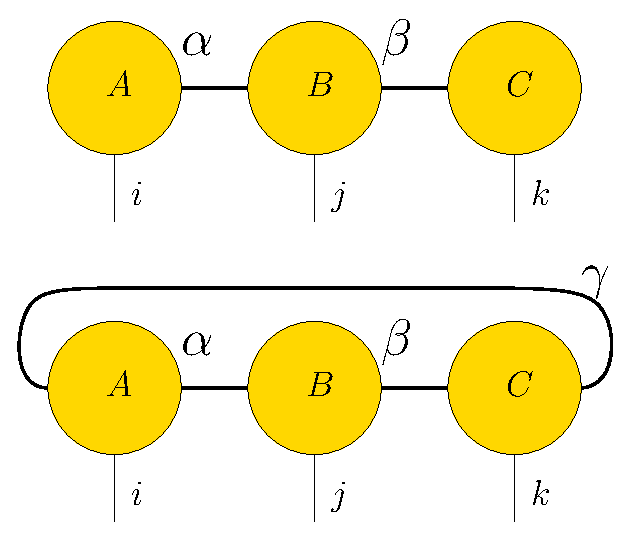
\includegraphics[width=.55\textwidth]{./Figures/mps-example.eps}
		\captionof{figure}{\textit{Two three-site MPS, the first lacking
		periodic boundary conditions and the second with periodic boundary conditions.}}
		\label{mps-example}
	\end{Figure}
	The indices $\chi_i$ in figure~\ref{mps-example} are called
	\textit{bond indices} and are associated with a
	\textit{bond dimension}. The free indices $i,j,k$ are
	\textit{site indices}. Algebraically, the MPS decomposition of a tensor $\Psi$ is written as:
	$$\Psi_{i_1,i_2,\cdots,i_N}=\sum_{\chi_1,\chi_2,\cdots,\chi_{N-1}}A^{[1]\chi_1}_{i_1}A_{i_2}^{[2]\chi_1,\chi_2}\cdots A^{[N]\chi_{N-1}}_{i_N}$$
	where the first and last local tensors $A^{[1]}$ and $A^{[N]}$ are
	matrices and every other tensor in the chain is of rank three. If
	each bond index is constrained to be of the same dimension $\chi$ then
	this representation approximates the $2^n$ coefficients of $\Psi$ using
	$$2\chi+(N-2)2\chi^2+2\chi=4\chi+(2N-4)\chi^2$$
	parameters, which grows as $O(N)$ for fixed $\chi$.
	For a given choice of site indices (e.g., $i_1=0$, $i_2=1$, $i_3=0$,
	$\cdots$), the coefficient $\Psi_{010\cdots}$ is given by a matrix
	product-- hence the name matrix product state.

	Consider a state $\ket{\Psi}\in\mathds{C}^{2\times\cdots\times2}$
	associated with N qubits.
	The \textit{Schmidt decomposition} of $\ket{\Psi}$ with respect to a
	partition of sites $A:B$ is written
	$$\ket{\Psi}=\sum_\alpha^{\chi_A}\lambda_\alpha\ket{\Phi_\alpha^{[A]}}\otimes\ket{\Phi_\alpha^{[B]}}$$
	where $\chi_A$ is the \textit{Schmidt rank} of the partition $A:B$
	and is a natural measure of the entanglement between the qubits in A
	and those in B~\cite{Vidal}. If $\max_A\chi_A=\chi$ and
	$$2^N>4\chi+(2N-4)\chi^2,$$
	then the MPS decomposition of $\ket{\Psi}$ with uniform bond
	dimension $\chi$ is exact and requires less memory than storing the
	individual $2^N$ coefficients of $\ket{\Psi}$.


	\subsection*{Generating a MPS from a tensor}
	The first step of the iterative process for generating a MPS from a
	tensor is depicted in figure~\ref{svd} for an initial tensor with
	three indices, each of dimension $d$. The input tensor $\psi$ is
	reshaped into a matrix $\psi_{MAT}$ by squashing indices the two
	leftmost indices into one index while keeping the rightmost index
	separated. The singular value decomposition is then performed on
	$\psi_{MAT}$. $\Sigma$ is truncated and renormalized to $\Sigma'$
	such that the bond index between $V$ and $\Sigma$ is less than or
	equal to the bond dimension $\chi$. The truncated matrix $\Sigma'$
	is contracted to the left into $U$, resulting in the $d^2\times\chi$
	matrix $\psi'_{MAT}$. Finally, the index of dimension $d^2$ is
	unsquashed into two indices of dimension $d$ each. The process is
	repeated for $\psi'$, with the only change being that the middle
	site index is squashed with the bond index and the leftmost site
	index is kept separate. This process is repeated iteratively for
	every site index in the original tensor $\psi$ until the tensor
	corresponding to the leftmost site is the only untouched tensor.
	See figure~\ref{mps-creation} for a depiction of this iterative
	process.
	\begin{Figure}
		\center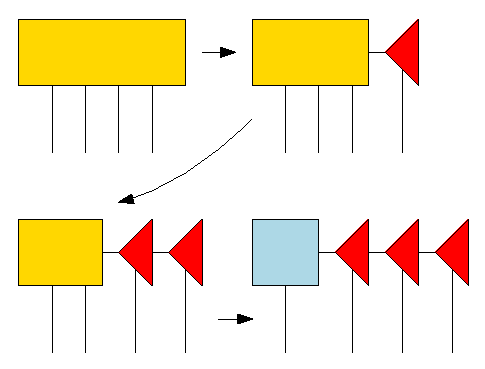
\includegraphics[width=.7\textwidth]{./Figures/mps-creation.eps}
		\captionof{figure}{\textit{How a MPS is generated using iterative SVD with
		an input tensor with four indices. Steps are numbered accordingly. The
		final orthogonality center is in blue.}}
		\label{mps-creation}
	\end{Figure}
	%%%%%%%% BREAK IN MULTICOL
	\end{multicols}
	\begin{Figure}
		\center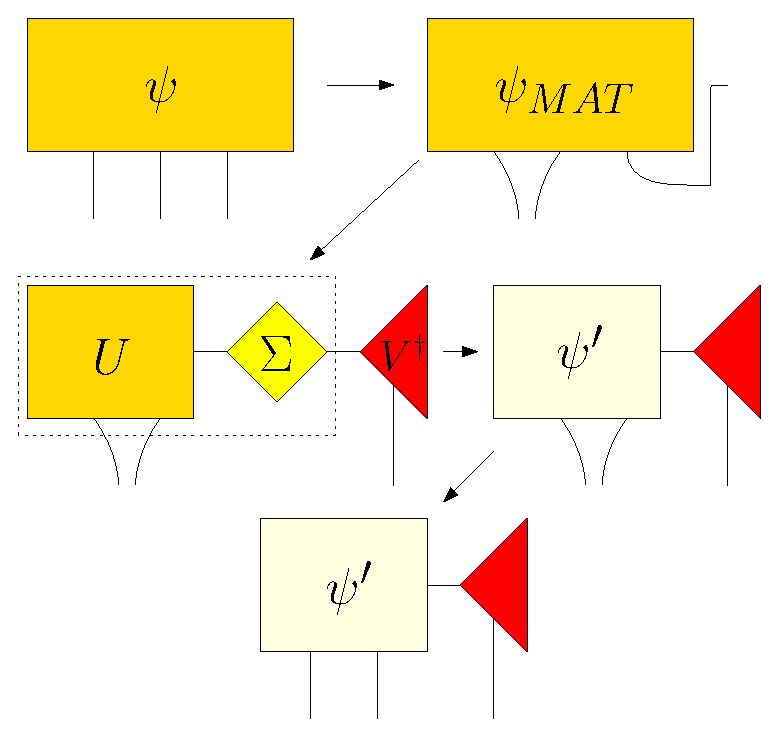
\includegraphics[width=.9\textwidth]{./Figures/svd.eps}
		\captionof{figure}{\textit{Separating the first site index from $\psi$.}}
		\label{svd}
	\end{Figure}
	\begin{multicols}{2}

	The leftmost site
	in figure~\ref{svd} is an orthonormal matrix by definition of the
	SVD. Non-boundary sites in the final chain resulting from
	iteratively applying this	method are \textit{right normal}, which is
	a loose generalization of orthonormality. Algebraically, if a tensor
	$T_{L,i,R}\in\mathds{C}^{b\times d\times b}$
	is right normal, then
	$$\sum_{i,R}T_{L,i,R}T^*_{L',i,R}=\delta_{L,L'}$$
	and likewise if $T$ is left normal then
	$$\sum_{i,L}T_{L,i,R}T^*_{L,i,R'}=\delta_{R,R'}.$$
	See figure~\ref{lr-normal} for a graphical depiction of this property.

	\begin{Figure}
		\center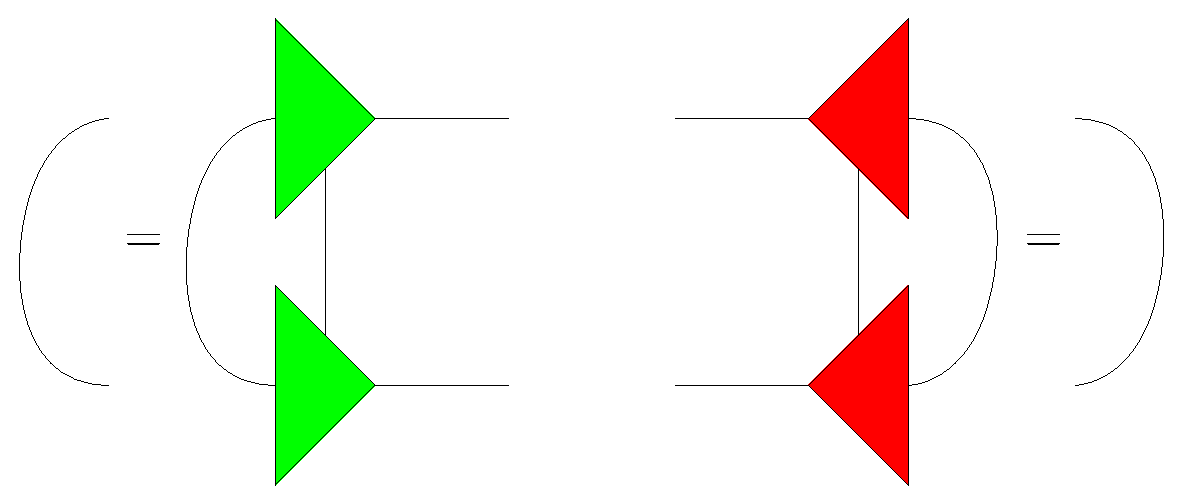
\includegraphics[width=.55\textwidth]{./Figures/lr_normal.eps}
		\captionof{figure}{\textit{Left normality (green) and right normality (red).}}
		\label{lr-normal}
	\end{Figure}

	If a MPS consists entirely of a nonnegative (possibly zero, as in
	figure~\ref{mps-creation}) number of left normal tensors facing a
	single unconstrained tensor followed by a chain of right normal
	tensors we call the single unconstrained tensor the
	\textit{orthogonality center}.


	\subsection*{Moving the Orthogonality Center}
	The orthogonality center presents a useful way of evaluating the
	expectation of a local operator $M$ on site $i$, depicted in
	figure~\ref{local-site-eval}.
	\begin{Figure}
		\center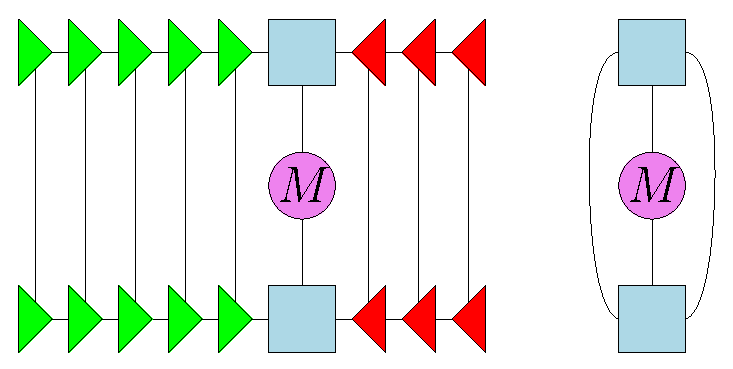
\includegraphics[width=.55\textwidth]{./Figures/local-site-eval.eps}
		\captionof{figure}{\textit{A quick way to find $\langle M^{(i)}\rangle_\psi$
		exploiting orthogonality. Left: the full contraction equivalent to
		$\bra{\psi_{MPS}}M^{(i)}\ket{\psi_{MPS}}$. Left and right normal tensors
		can be removed, leaving the contraction on the right as the only
		necessary computation.}}
		\label{local-site-eval}
	\end{Figure}
	However, this requires that the orthogonality center is already
	located on site $i$. Since this clearly will not always be the case,
	we need a way to move the orthogonality center from one site to another.
	The general idea is depicted in figure~\ref{moving-ortho-center}.
	Briefly, the orthogonality center's site index is squashed with the
	left (right) bond index. Next it is split into two matrices
	using the QR (LQ) decomposition, and the left (right) normal matrix
	is reshaped into a rank three tensor. The remaining matrix is
	contracted into the corresponding right (left) neighbor tensor.

	\begin{Figure}
		\center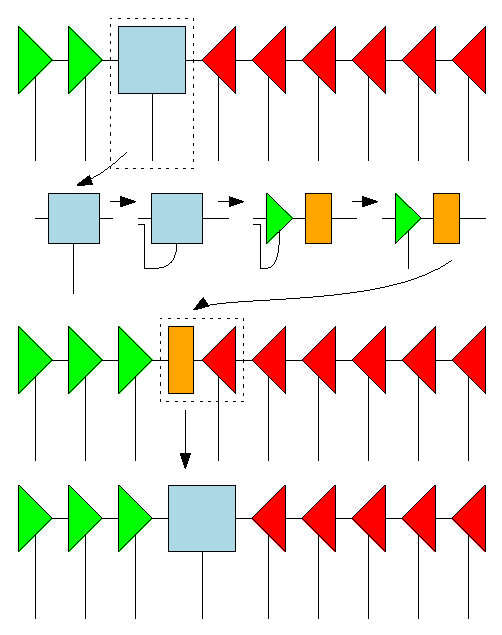
\includegraphics[width=.7\textwidth]{./Figures/move-ortho-center.eps}
		\captionof{figure}{\textit{Moving the orthogonality center one site
		 to the right using the QR factorization. This can be repeated to
		 move the orthogonality center to any site to the right of its
		 current position. To move the orthogonality center to the left,
		 a similar process is used substituting the LQ factorization for
		 the QR factorization.}}
		\label{moving-ortho-center}
	\end{Figure}


	\subsection*{Time Evolving Block Decimation}
	Time evolving block decimation (TEBD) is a method for efficiently
	simulating 1D quantum systems with low entanglement. By leveraging
	the fidelity of the system's MPS decomposition, a
	Suzuki-Trotter~\cite{suzuki}
	decomposition of the propogator
	$$\hat{U}(t)=\exp\{-i\hat{H}t/\hbar\}$$
	can be applied step-by-step to the MPS with bond dimensions truncated
	after each step. For the 1-D transverse field Ising model
	$$\hat{H}=\sum_{i=1}^{N-1}\sigma_z^{(i)}\sigma_z^{(i+1)}+J\sum_{i=1}^N\sigma_x^{(i)}$$
	this amounts to applying $p$ Trotterized operators (setting $\hbar=1$):
	\[
		\hat{U}(t) =
		\left[
			\left(\prod_{i=1}^{N-1}
				e^{-i\sigma_z^{(i)}\sigma_z^{(i+1)}\Delta t}
			\right)
			\left(\prod_{i=1}^Ne^{-i\sigma_x^{(i)}\Delta t}\right)
		\right]^p
	\]
	where the step size $\Delta t=\frac{t}{p}$. A depiction of one TEBD
	sweep with this Hamiltonian is shown in figure~\ref{TEBD}.

	\begin{Figure}
		\center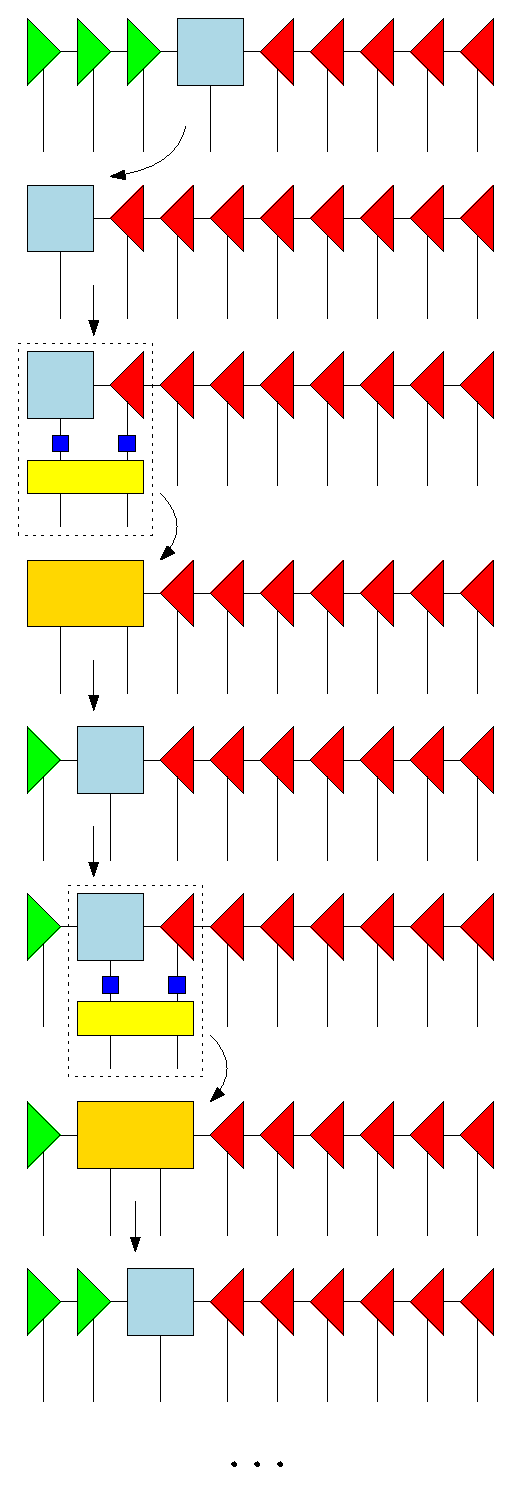
\includegraphics[height=350pt]{./Figures/tebd.eps}
		\captionof{figure}{\textit{One step of time evolving block
		decimation. The orthogonality center is moved to the leftmost site.
		Trotterized operators $R_x(\Delta t)$ in blue and $R_{zz}(\Delta t)$
		in yellow are
		applied to the orthogonality center and its rightmost neighbor. A
		SVD is performed and the singular value matrix is truncated and
		contracted to the right to enforce the bond dimension $\chi$. The
		sweep continues until reaching the last site, at which
		point the orthogonality center is again moved to the leftmost site
		and the above process is repeated $p-1$ additional times.}}
		\label{TEBD}
	\end{Figure}

	This approximation is not sufficient when the Hamiltonian $\hat{H}$
	generates sufficiently high entanglement, since enforcing the
	maximum bond dimension $\chi$ bounds the maximum amout of
	entanglement the MPS can ever reach. If, however, $\hat{H}$ consists
	entirely of single-site terms, then this method is exact since the
	systems entanglement cannot grow through time evolution under
	$\hat{H}$. See the rightmost heatmap in figure~\ref{tebd-heatmaps}
	for an example of what time evolution under a nonentangling
	Hamiltonian might look like.


\section*{Package Overview}
	This section provides an overview of the real core of this project: a
	Julia package for creating and manipulating matrix
	product states, located at~\\
	\url{https://github.com/gl3nnleblanc/pdrp2021}.
	\subsection*{Julia}
	Julia is a modern programming language incubated at MIT in 2009 and
	designed from the beginning with high performance in mind~\cite{Julia-lang}.
	Julia is fast, easy to use, and open source.
	\subsection*{Algorithms}
	The following section contains pseucode outlining the main ideas
	of what was implemented in the package. Again, the full code written
	in Julia is available at the repository.
	\begin{algorithm}[H]
		\KwData{input tensor $T$, left\_dim, right\_dim, $\chi$}
		\KwResult{length($\Sigma$), $T_{next}$, $V$}
		$T_{MAT}$ $\mapsfrom$ reshape(T, left\_dim, right\_dim)\;
		$T_{next}$, $\Sigma$, $V^\dagger$ $\mapsfrom$ SVD($T_{MAT}$)\;
		$V$ $\mapsfrom$ $(V^\dagger)^\dagger$\;
		$\Sigma$ $\mapsfrom$ truncate\_to\_chi($\Sigma$, $\chi$)\;
		$T_{next}$ $\mapsfrom$ truncate\_to\_chi($T_{next}$, $\chi$)\;
		\Return length($\Sigma$), $T_{next}$, $V$\;
		\caption{Helper function for splitting a tensor.}
		\label{split-tensor}
	\end{algorithm}
	\vspace{20px}
	\begin{algorithm}[H]
		\KwData{input tensor $\Psi$, desired bond dimension $\chi$}
		N $\mapsfrom$ tensor rank of $\Psi$\;
		sites $\mapsfrom$ [ ]\;
		$d_{next}$, $T_{next}$, $T_{curr}$ $\mapsfrom$ split\_tensor($\Psi$, $2^{N-1}$, 2, $\chi$)\;
		sites.append($T_{curr}$)\;
		\For{i $\mapsfrom$ 2 to $N-1$}{
			$d_{next}$, $T_{next}$, $T_{curr}$ $\mapsfrom$ split\_tensor($T_{next}$, $2^{N-i}$, $2^i$, $\chi$)\;
			\eIf{length($T_{curr}$) = $\chi^2$ * 2}{
				$T_{curr}$ $\mapsfrom$ reshape($T_{curr}$, $\chi$, 2, $\chi$)\;
			}{
				$d_{prev}$ $\mapsfrom$ length($T_curr$) $\div$ $(2 \times d_{next})$\;
				$T_{curr}$ $\mapsfrom$ reshape($T_{curr}$, $d_{next}$, 2, $d_{prev}$)\;
			}
			sites.append($T_{curr}$)\;
		}
		\_, $T_{next}$, $T_{curr}$ $\mapsfrom$ split\_tensor($T_{next}$, 2, $d_{prev}$, $\chi$)\;
		$T_{curr}$ $\mapsfrom$ reshape($T_curr$, 2, 2, :)\;
		sites.append($T_{curr}$)\;
		sites.append($T_{next}$)\;
		\Return MPS(sites, $\chi$, N)\;
		\caption{Generating a MPS from input tensor $\Psi$.}
		\label{mps-gen}
	\end{algorithm}

		Algorithm~\ref{mps-gen} returns a MPS wrapper consisting of an array of
		tensors arranged from left to right in descending order. Said another way,
		the $N$th entry of this array is the leftmost site.

	%TODO: orthogonality center moving pseudocode
	%TODO: single tebd sweep pseudocode
	%TODO: tebd evolution pseudocode
	\subsection*{Examples}
	There are three example notebooks contained in the repository (as
	linked above). Some highlights:

	\begin{Figure}
		\center
\includegraphics[height=100px]{./Figures/lenna-chi-2.png}
		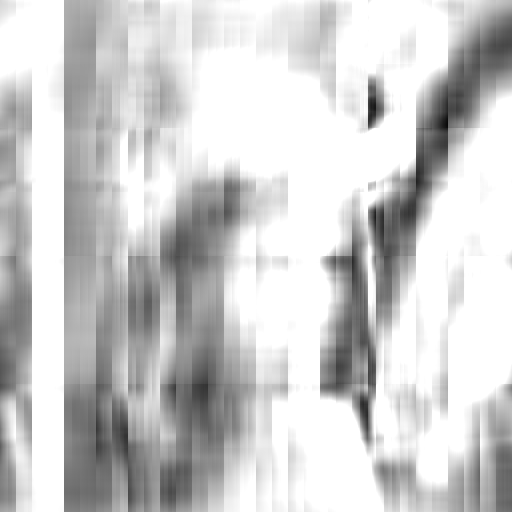
\includegraphics[height=100px]{./Figures/lenna-chi-9.png}\\
		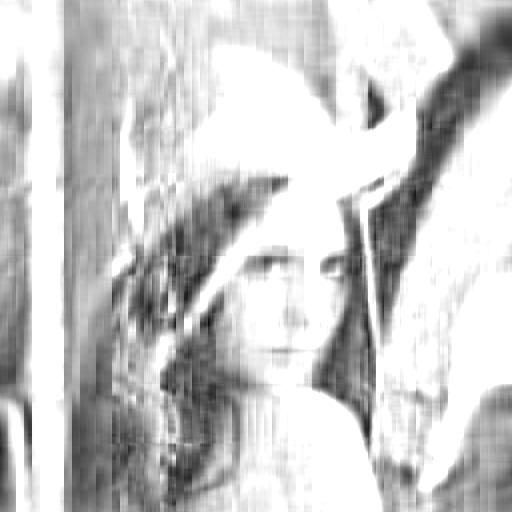
\includegraphics[height=100px]{./Figures/lenna-chi-20.png}
		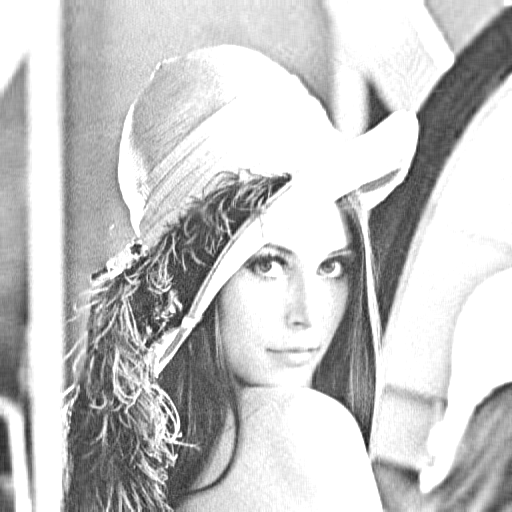
\includegraphics[height=100px]{./Figures/lenna-chi-100.png}
		\captionof{figure}{\textit{Compressing an image with an MPS.
		Clockwise from top left: $\chi=2$, $\chi=9$, $\chi=20$, $\chi=100$,
		with compression ratios of 1927.5, 126.2, 31.3, and 2.24,
		respectively. Lossless storage as a MPS results in a compression ratio
		less than 1.}}
		\label{lenna-compression}
	\end{Figure}

	\begin{Figure}
		\center
\includegraphics[height=200px]{./Figures/ising_j1_interactions_heatmap.png}\hspace{50px}
\includegraphics[height=200px]{./Figures/ising_j1_local_heatmap.png}
		\captionof{figure}{\textit{Heatmaps of $\langle\sigma_z\rangle$ for each
		site in a chain of 12 qubits time evolving under a ($J=1$) 1D Ising model with (left) and without (right) the local interaction term
		$\sigma_z^{(i)}\sigma_z^{(i+1)}$. Using an MPS with $\chi=32$ and
		running 1000 sweeps on an Intel i5-6600k @ 3.9 GHz took $\approx3$ minutes.}}
		\label{tebd-heatmaps}
	\end{Figure}

	\begin{Figure}
		\center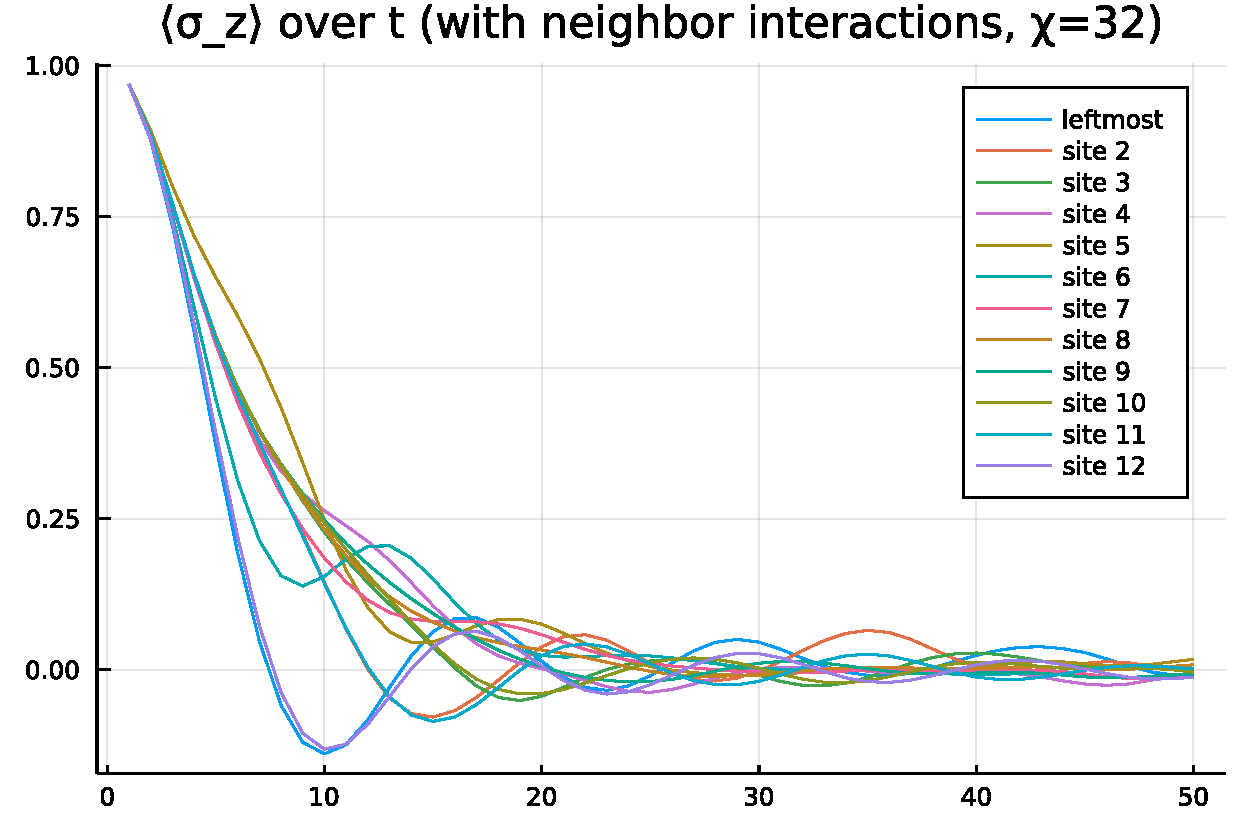
\includegraphics[width=0.9\textwidth]{./Figures/ising_with_interactions.pdf}
		\captionof{figure}{\textit{Graph corresponding to the left heatmap in figure~\ref{tebd-heatmaps}.}}
		\label{tebd-graphs}
	\end{Figure}



	\subsection*{Next Steps}
	This project felt extremely rewarding and I'm planning to continue
	sporadically adding things to it over the summer when I have the
	time. Two things that I'd like to implement are DMRG~\cite{DMRG}
	and a neural network using a MPS whose sites correspond to lifted
	features~\cite{mps-ml},~\cite{Huggins}.


\bibliography{./references}

\end{multicols}


\end{document}
